\chapter[Backgrounds to $\Htautau$][Backgrounds to $\Htautau$]{Backgrounds to $\Htautau$}
\label{chap:results}

\begin{quote}
Background estimates in the $\Htautau$ analysis are described.
\end{quote}

\section{$j \rightarrow \tauh$ mis-identification}
\label{sec:backgrounds-misid}

\begin{figure}[tp]
  \centering
  \includegraphics[width=0.48\textwidth]{figures/backgrounds/jetBDT-1p}
  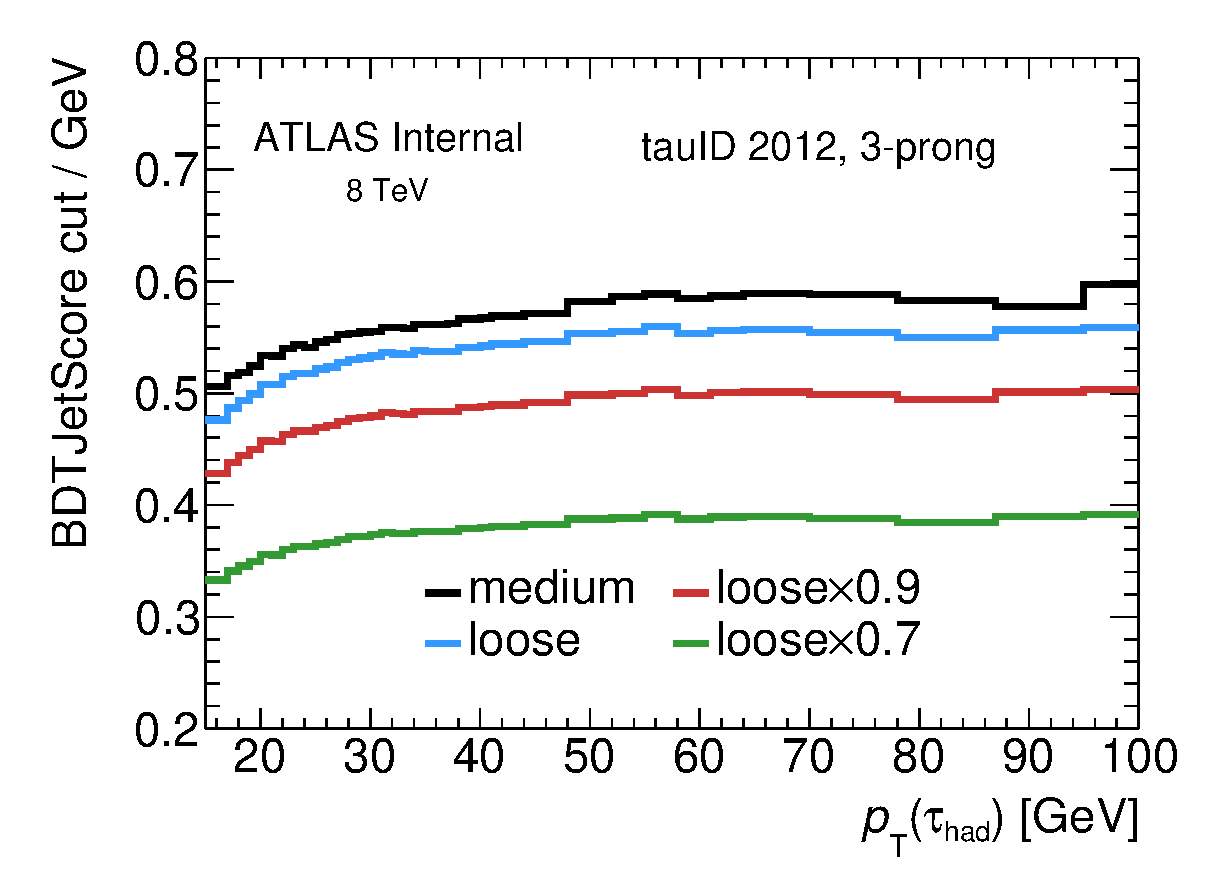
\includegraphics[width=0.48\textwidth]{figures/backgrounds/jetBDT-3p}
  \caption{Variables.}
  \label{fig:backgrounds-workingpoints}
\end{figure}

\begin{figure}[tp]
  \centering
  \includegraphics[width=0.48\textwidth]{figures/backgrounds/fakefactor_8TeV_boosted_1p_CRs}
  \includegraphics[width=0.48\textwidth]{figures/backgrounds/fakefactor_8TeV_boosted_1p_mix}
  \caption{Variables.}
  \label{fig:backgrounds-fakefactorsboost1p}
\end{figure}

\begin{figure}[tp]
  \centering
  \includegraphics[width=0.48\textwidth]{figures/backgrounds/fakefactor_8TeV_boosted_3p_CRs}
  \includegraphics[width=0.48\textwidth]{figures/backgrounds/fakefactor_8TeV_boosted_3p_mix}
  \caption{Variables.}
  \label{fig:backgrounds-fakefactorsboost3p}
\end{figure}

\begin{figure}[tp]
  \centering
  \includegraphics[width=0.48\textwidth]{figures/backgrounds/fakefactor_8TeV_vbf_1p_CRs}
  \includegraphics[width=0.48\textwidth]{figures/backgrounds/fakefactor_8TeV_vbf_1p_mix}
  \caption{Variables.}
  \label{fig:backgrounds-fakefactorsVBF1p}
\end{figure}

\begin{figure}[tp]
  \centering
  \includegraphics[width=0.48\textwidth]{figures/backgrounds/fakefactor_8TeV_vbf_3p_CRs}
  \includegraphics[width=0.48\textwidth]{figures/backgrounds/fakefactor_8TeV_vbf_3p_mix}
  \caption{Variables.}
  \label{fig:backgrounds-fakefactorsVBF3p}
\end{figure}


